%%%%%%%%%%%%%%%%%%%%%%%%%%%%%%%%%%%% --Master File--- %%%%%%%%%%%%%%%%%%%%%%%%%%%%%%%%
%%% Time-stamp: <2020-08-28 05:00:00 Chandra Has>
%%% Document class is beamer
%%% Document is using theme ChPresentation v1.1 <2020-08-28 05:00 Chandra Has>
%============================= Document class and theme ================================
% Documment class
\documentclass[aspectratio=169]{beamer}
%\usepackage{CJKutf8}
%\usepackage[number]{natbib}

\usepackage[T1]{fontenc}
\usepackage[scaled]{helvet} % close to Arial
%\usepackage{newtxmath,newtxtext} % Times New Roman

\definecolor{highlightgreen}{HTML}{70AD47}
\definecolor{highlightblue}{HTML}{004DD6}
\definecolor{highlightred}{HTML}{C00000}
\newcommand\highlightblue{\textcolor{highlightblue}}
\newcommand\highlightred{\textcolor{highlightred}}
\newcommand\highlightgreen{\textcolor{highlightgreen}}

% Beamer theme
\usetheme[footline, progressbar=fraction]{ChPresentation}
%\usetheme[conference, darkblue, headline, footline, progressbar=percent]{ChPresentation}

%-----------------------------------------------------------------------
%        Title page: titlepage (default), notitlepage
% 	   	 Title styles: plain (default), seminar, conference
%		 Color themes: darkred (default), darkblue, darkgreen
%		 Header/footer: headline, footline
% 		 Progress bar styles: progressbar=fraction, progressbar=percent
%        Frame logo position: logtoprightside (default), backgroundlogo
%		 Vertical alignment: t (default), c
%------------------------------------------------------------------------

%\progressbar[red]{yellow}
%\framebackgroundlogoopacity[0.2]
%\backgroundcanvas{\includegraphics[width=\paperwidth, height=\paperheight]{bg1}}

%============================= Packages and other commands ================================
% Graphics paths
\graphicspath{{assets/}{logos/}}
%\linespacing[1.12] 

%============================== Title page information =====================================
%%%%% Predefined %%%%%  
\title[Beamer Presentation: Various Links]{HAI Course Project Presentation}
\subtitle{Your Project Name}

\author{Authors\\Date}

\institute{AI Thrust\\
HKUST (GZ)}

%\date[\today]{\scriptsize \today}

\titlegraphic{
\includegraphics[scale=0.07]{logos/HKUSTGZ.png}}
%\logo{\includegraphics[scale=0.08]{logo}}

%%%%% Custom %%%%%
\framelogo{
\includegraphics[scale=0.047]{logos/HKUSTGZ.png}} 

%***********************************Main body*******************************************
\begin{document}

%---------------------------------------------------------------------------------------	
\backgroundcanvas{}
%--------------------------------------------------------------------------------------

%---------------------------------------------------------------------------------------
\section[Outline]{}
%--------------------------------------------------------------------------------------

%======================================
% Use \begin{frame}[allowframebreaks]{Title}
% if the TOC does not fit in one frame.
\begin{frame}{Table of Contents}
	\tableofcontents
\end{frame}
%====================================== 

%---------------------------------------------------------------------------------------

\section{Section Name 1}

\begin{frame}[fragile]{Section Name 1}
Title
\begin{itemize}
\item item\\
\vspace{-5pt}
\item item\\
\end{itemize}
\end{frame}

\section{Section Name 2}

\begin{frame}[fragile]{Section Name 2}
Title
\vspace{-15pt}
\begin{columns}
\begin{column}{0.46\textwidth}
\begin{itemize}
\item item
\vspace{-5pt}
\item item
\vspace{-5pt}
\item item
\end{itemize}
\end{column}
\begin{column}{0.54\textwidth}
\begin{itemize}
\item item
\vspace{-5pt}
\item item
%\vspace{-5pt}
%\item GAMES研讨会2021
\end{itemize}
\end{column}
\end{columns}
\end{frame}

\begin{frame}[fragile]{Section Name 2}
\vspace{-12pt}
\centering{\highlightred{Title}}\\
\begin{columns}
\column{0.6\linewidth}
\begin{cblock}{\centering Test Image}
\centering
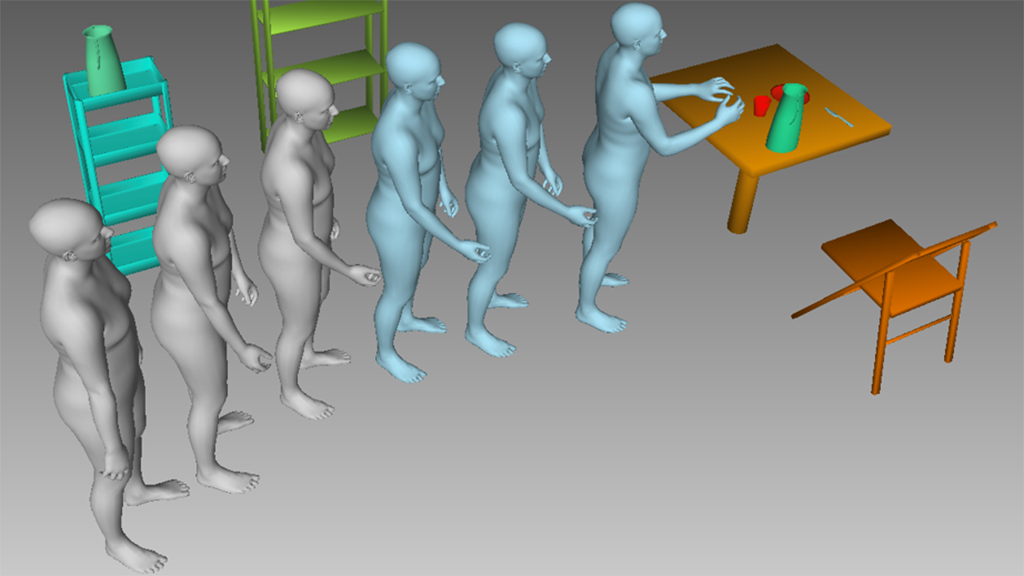
\includegraphics[width=\linewidth]{assets/hoimotion_thumb.png}
\cite{hu24hoimotion}
\end{cblock}
\end{columns}
\end{frame}

\begin{frame}[fragile]{Section Name 2}
\vspace{-12pt}
\centering{\highlightred{Title}}\\
\begin{columns}
\column{0.45\linewidth}
\begin{cblock}{\centering Test Image 1}
\centering
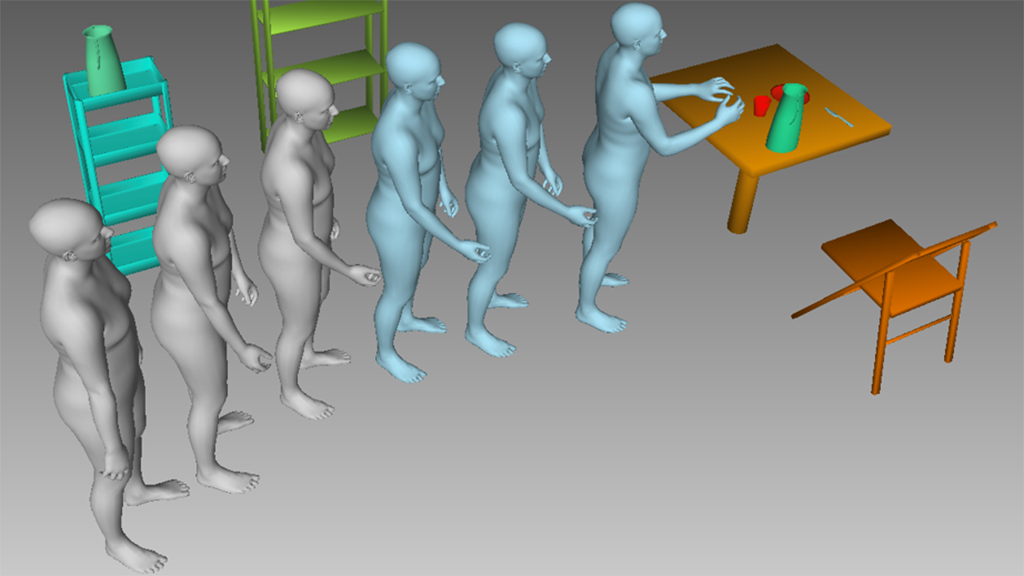
\includegraphics[width=\linewidth]{assets/hoimotion_thumb.png}
\cite{hu24hoimotion}
\end{cblock}
\column{0.45\linewidth}
\begin{cblock}{\centering Test Image 2}
\centering
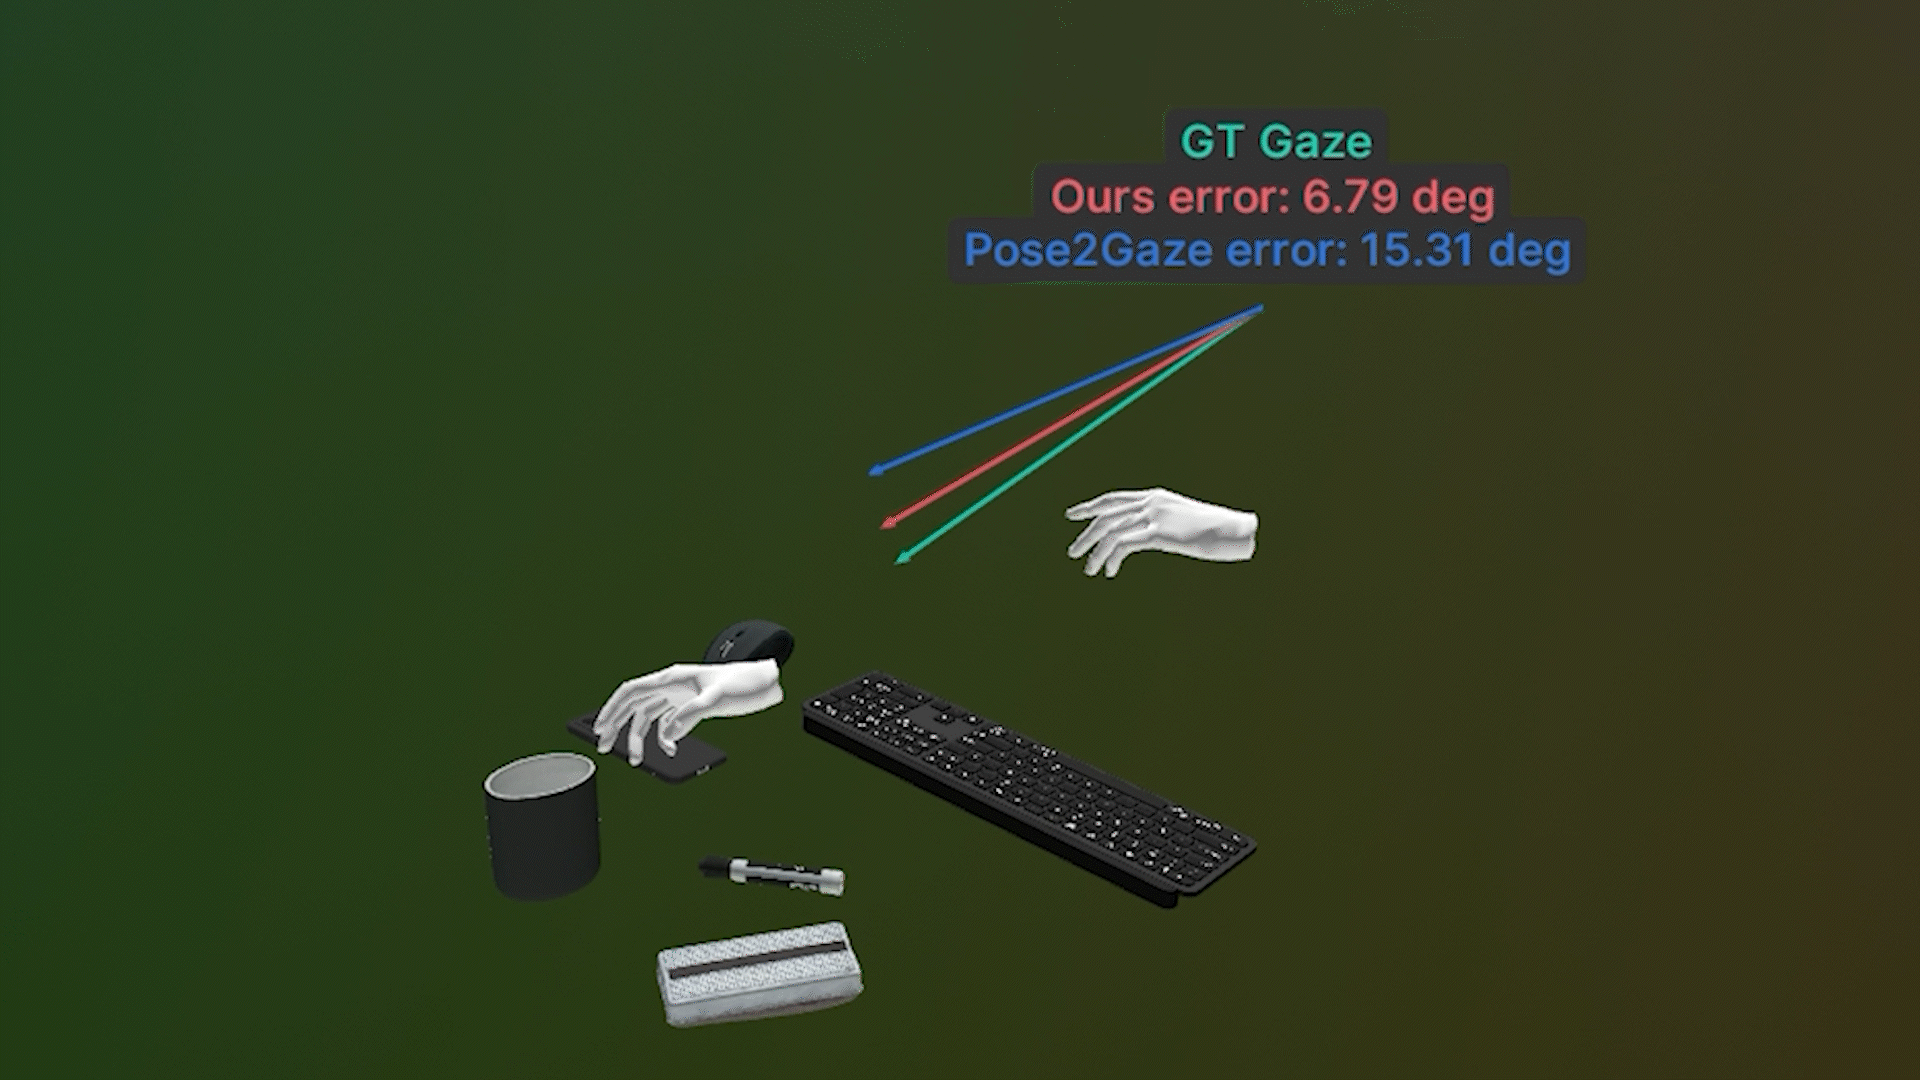
\includegraphics[width=\linewidth]{assets/hoigaze_thumb.png}
\cite{hu25hoigaze}
\end{cblock}
\end{columns}
\end{frame}

\begin{frame}[fragile]{Conclusion}
\begin{columns}[t]
    \column{0.3\linewidth}		
    \begin{block}{\centering Conclusion 1}
        \centering{            
        \begin{enumerate}
            \item item
            \item item
            \item item
        \end{enumerate}}
    \end{block}

    \column{0.3\linewidth}		
    \begin{exampleblock}{\centering Conclusion 2}
        \centering{            
        \begin{enumerate}
            \item item
            \item item
            \item item
        \end{enumerate}}
    \end{exampleblock}
    
    \column{0.3\linewidth}		
    \begin{alertblock}{\centering Conclusion 3}
        \centering{            
        \begin{enumerate}
            \item item
            \item item
            \item item
        \end{enumerate}}
    \end{alertblock}        		
\end{columns}
\end{frame}

\begin{frame}
\vspace{80pt}
\centering
{
  Thank you!\\  
  Any questions?
}
\begin{columns}[t]
\end{columns}
%	\scriptsize	
\end{frame}

\begin{frame}[allowframebreaks]{References}
\bibliographystyle{abbrvnat}
{\tiny
  \bibliography{ref}
}
\end{frame}

\end{document}
%===========================================================================================